\graphicspath{ {project_images/} }

\section{Methods}

The SVM, CNN, ResNet50, and VGG16 classifiers were implemented for our project.
Below, we will describe the algorithms we used in detail.

\subsection{SVM}
SVM operates by defining a division line between classes using a kernel function. 
The chosen kernel function, uses parameters $C$ and $\gamma$ to perform the calculation to separate the dataset into their respective classes.
In our case, we converted the images to arrays to allow SVM to process our dataset.
Before feeding the dataset, it is imperative to have the dataset standardized.
We decided to standardize it using MinMaxScaler, as StandardScaler would change the data to be within the range $[0,1]$.
This took extra time to process, and ultimately yielded no significant improvement in performance.
By implementing a Pipeline, we were able to consolidate the code and concisely read the process being done by the program.
Also, by using GridSearch, we were able to let the SVM classifier run with a K-Fold comparison added to find the best performing model.

\begin{figure}[h]
	\centering
	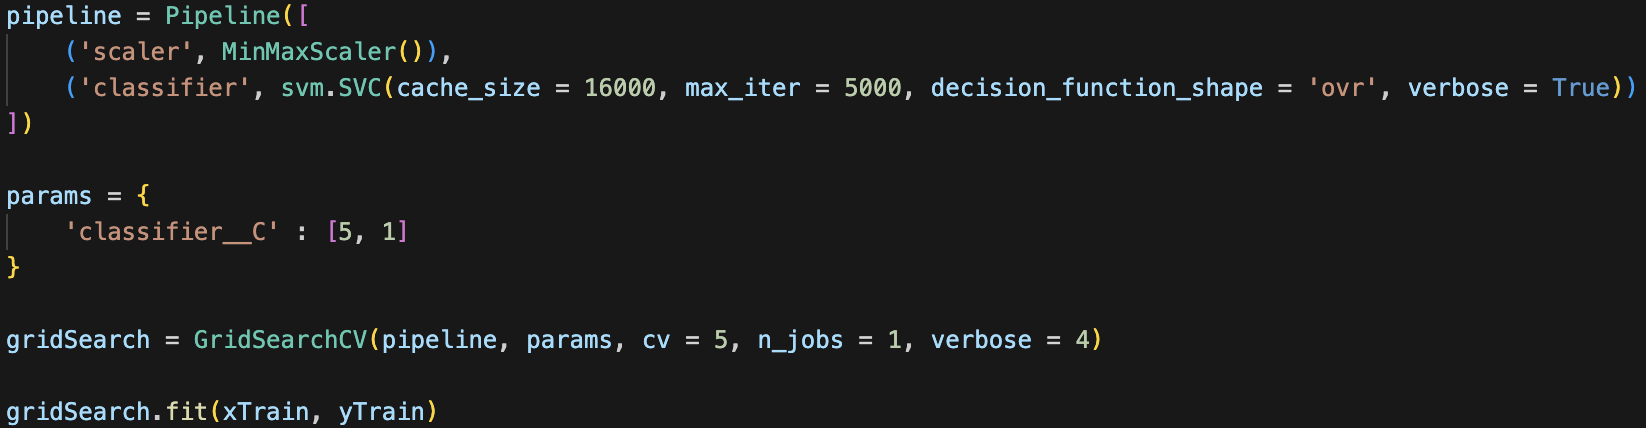
\includegraphics[scale=0.5]{SVM_explained.png}
	\caption{SVM using Pipeline and Grid Search within the Jupyter Notebook}
	\label{fig:figure1}
\end{figure}

\subsection{CNN}
Convolutional Neural Networks (CNN) is commonly used for image classification tasks. Typically, CNN models consist of convolutional layers that apply filters to extract features and patterns, pooling layers to retain the important features and patterns, and fully connected layers to make predictions based on the features learned in the convolutional and pooling layers \cite{CNNGuide}.
Our CNN model implements a sequential structure, where the layers are added linearly. The input layer takes in the parameters of the image, in our case our images were 500x500 pixels with a color channel of 1 (since they are greyscale images). After input, the first convolutional layer applies filters to capture the features in the image data by moving a matrix of learnable weights over the image. In our model, the filters had a size of 3x3 and the number of filters increased in each convolutional layer. At the beginning of training, the weights are random before adapting its value throughout the training process. The extracted features are put into a feature map that the following pooling layer uses to further extract important features. Our model uses max-pooling, which looks for the maximum value extracted by each filter from the previous layer so that the initial feature map is downsampled. This pattern of convolutional layer followed by pooling layer iterates to continue extracting features and downsampling the feature map before a flatten layer reshapes the feature map into a one-dimensional vector that can be inputted into a fully connected dense layer. The convolutional layers and max-pooling layers iterate 3 times in our model before the feature map is flattened. We found that less iterations yielded poorer performance (model was not complex enough) and more iterations resulted in longer training time (model was more complex and computational load was larger). The dense layer is considered a "fully connected" layer because each neuron in a dense layer is connected to every extracted feature and is assigned a weight value. The initial weights are random but are learned throughout the training process. The weight of each of the connections in the dense layer attempt to understand the relationship between the important features extracted from the previous layers as a representation of a prominent feature. The output layer is a dense layer with neurons equal to the number of classes in the dataset; in our case there are 3 classes (cat, dog, and panda). The summary of the structure of our CNN model is shown in Figure \ref{fig:figure1} below.

\begin{figure}[h]
	\centering
	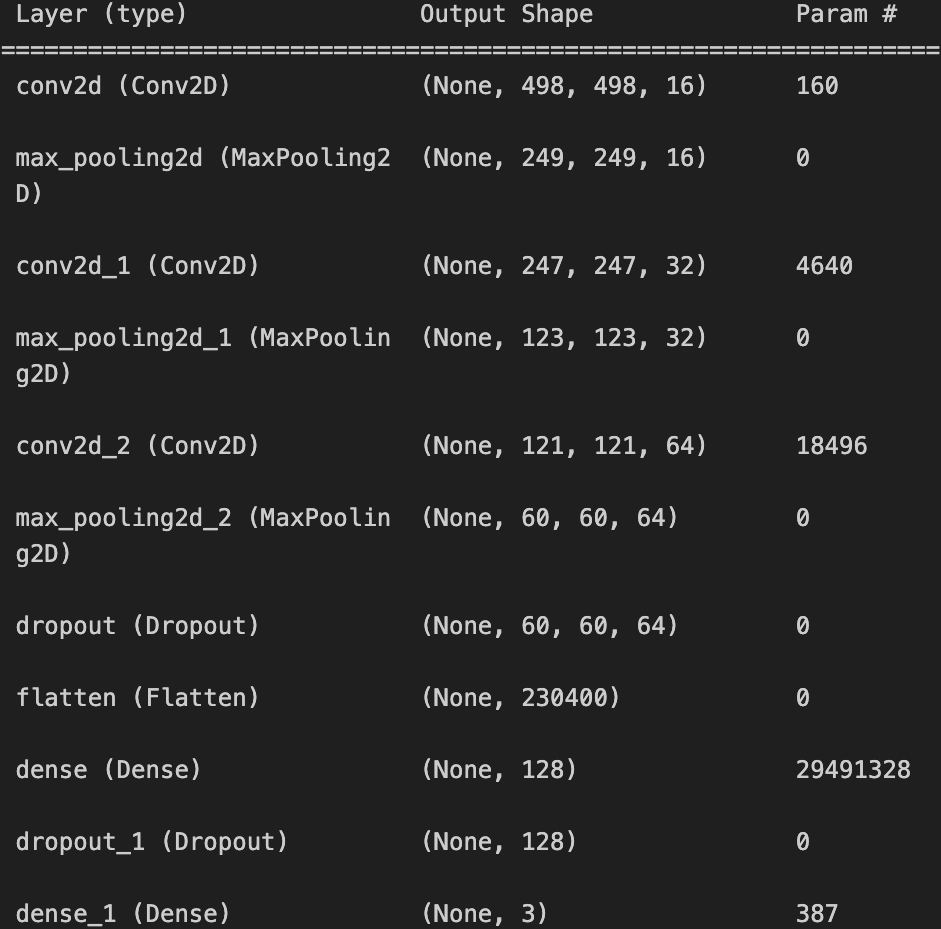
\includegraphics[scale=0.5]{CNN_structure}
	\caption{CNN model summary.}
	\label{fig:figure1}
\end{figure}

Our convoluted layers use the Rectified Linear Unit (ReLu) activation function to introduce non-linearity, this way our model can learn complex relationships between the features of our data. The ReLu activation function sets negative values found in the convolution matrix to 0, allowing the model to focus on the positive values that likely represent relevant features. In between the dense layers, we implemented dropout regularization to prevent overfitting. Dropout works by temporarily setting the weights of a random set of neurons to 0 ("dropping out") per epoch. This prevents overfitting by forcing the model to learn more robustly instead of relying too much on the recognition of certain features and "memorizing" the training data. The output dense layer uses the Softmax activation function to scale the numerical output of the model into probabilities distributed over the possible output classes represented by indexes. The class with the highest probability is considered the predicted class which is mapped to the string value of the class using the index value.

While fitting the model, we implemented the EarlyStopping callback to reduce the likelihood of overfitting by stopping training if the validation accuracy did not improve after 5 consecutive epochs. The EarlyStopping callback can also be useful in preventing underfitting if the number of epochs is set to a higher number than what is expected to be necessary. 

\subsection{ResNet50}

Residual Network 50 (ResNet50) is a type of CNN algorithm that contains 50 hidden layers. 
This algorithm allows for the use of Convolution2D and MaxPooling2D layers just like the standard CNN algorithm.
The 'Residual' portion refers to how the gradient is handled within the structure of the algorithm itself.
The gradient is the result calculated from the partial derivatives of the loss function, with respect to the given data's parameters \cite{Gradient}.
Instead of using standard back-propogation, it has a separate structure called a residual block which allows for the gradient to flow more easily through the entire structured network\cite{RN50}.

\begin{figure}[h]
	\centering
	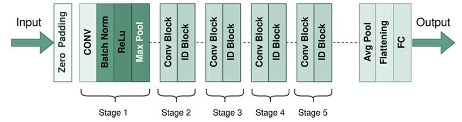
\includegraphics[scale=0.5]{ResNet_structure.jpg}
	\caption{A sample structure of the Res Net 50 Algorithm}
	\label{fig:figure5}
\end{figure}

\subsection{VGG16}
VGG16 is a pre-trained CNN model available for use through Tensorflow. VGG16 was pre-trained for image classification on large datasets such as ImageNet where the input image size was 224x224 pixels with 3 color channels (RGB). Its structure consists of 13 convoluted layers and 3 fully connected dense layers (16 layers total) \cite{VGG16Explained}. We decided to use a pre-trained VGG16 model instead of building one from scratch to learn how efficiently it would execute our particular image classification task. 
To utilize the pre-trained VGG16 model, we first load the base model without the top layers as these layers are what we need to modify to have the model classify our cat, dog, and panda images. Initially, the custom layers we added included 3 fully connected dense layers; however, we found the training time to be especially long and after experimenting with removing a dense layer to make the model less complex, we found that the training time was shortened with very little change in performance. Ultimately, we chose to keep working with the shortened training time with two dense layers. The first dense layer utilizes ReLu activation as well as the He uniform kernel initializer to initialize the weights of the 64 neurons within a uniform range dependent on the number of input neurons. He uniform combats the possibility of too many dead neurons by increasing the likelihood that neurons will activate and not be stuck in an inactive state throughout the entirety of training. This gives more neurons the chance to contribute to learning. The structure of the pre-trained VGG16 is shown in \ref{fig:figure2} below. The last output dense layer acts the same as it did in our previous CNN model, utilizing Softmax to generate probabilities distributed over the three output classes mapped to their corresponding string values. 

\begin{figure}[h]
	\centering
	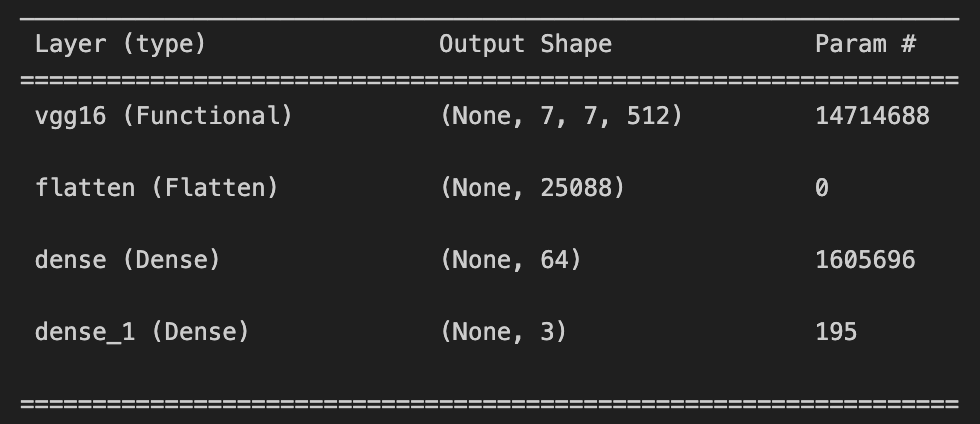
\includegraphics[scale=0.5]{VGG16_structure}
	\caption{Pre-trained VGG16 model summary. The base model is loaded and the top dense layers are added manually.}
	\label{fig:figure2}
\end{figure}